\documentclass{article}
\usepackage[utf8]{inputenc}
\usepackage[a4paper,top=2cm,bottom=2cm,left=2cm,right=2cm,marginparwidth=1.75cm,headheight=28pt]{geometry}
\usepackage[utopia]{mathdesign}
\usepackage{graphicx}
\usepackage{siunitx}
\usepackage{amsmath}
\usepackage{cancel}
\title{Apunte Termodinámica}
\author{Patricio Whittingslow}
\date{Abril 2019}
\newcommand{\ctegas}{k}
\newcommand{\cte}{\textrm{cte}}
\newcommand{\cp}{c_{p}}
\newcommand{\cv}{c_{v}}
\newcommand{\snaught}{s^{0}}
\newcommand{\agitacion}{\textrm{Agit.}}
\newcommand{\inicial}{i}
\newcommand{\Sgen}{S_{\textrm{gen}}}
\newcommand{\sib}[1]{[\si{#1}]}
\newcommand{\final}{f}
\newcommand{\rc}{r_c}
\newcommand{\rp}{r_{\mbox{\scriptsize$p$}}}
\newcommand{\rv}{r_{\mbox{\tiny$V$}}}
\newcommand{\util}{{\textrm{útil}}}
\newcommand{\Wutil}{W_{ \footnotesize \util}}
\newcommand{\Qaport}{Q_{\footnotesize\textrm{aportado}}}
\newcommand{\aislado}{\textrm{Ais.}}
\newcommand{\Boltzmann}{k_{\textrm{B}}}
\newcommand{\Qextr}{Q_{\footnotesize\textrm{extraído}}}
\newcommand{\moldens}{\bar{n}}
%% Macros
\newcommand{\spartial}[2]{\frac{\partial #1}{\partial #2}}
\newcommand{\dpartial}[2]{\frac{\partial^2 #1}{\partial #2^2}}

\newcommand{\di}{\textrm{d}}
 \mathchardef\mhyphen="2D
 \newcommand{\hyph}{\,\mhyphen}
 \newcommand\numberthis{\addtocounter{equation}{1}\tag{\theequation}}
\begin{document}

\maketitle
\section{Principios}
\subsection{Principio de estado}
Cuantas variables se necesitan para describir el estado termodinámico de un sistema?
\begin{itemize}
    \item[$N$] Número de variables independientes
    \item[$n$] Número de formas pertinentes de intercambiar trabajo
\end{itemize}
\[
N= n + 1
\]

\section{ Gases Ideales }
Ley de los Gases Ideales
\[p  = \moldens \Boltzmann T= \frac{N\tilde{R}T}{V}
\]
donde $N$ es la cantidad de moles, $\tilde{R}=8.314\, \si{\joule \per \kelvin\per \mole}$ es la constante universal de gases ideales, $R$ es la constante especifica de un gas ideal, $\moldens$ es la cantidad de moléculas de gas por metro cuadrado y $\Boltzmann$ es la constante de Boltzmann $\Boltzmann=\SI{1,38e-23}{\meter \squared \kilogram \per \second \squared \per \kelvin}$. Existe también la expresión especifica para la ley:
\[
p = \frac{RT}{v}=\rho RT
\]
donde $R$ \sib{\joule \per \kilogram \per \kelvin} es la constante especifica del gas con el cual se trabaja y $v=\frac{1}{\rho}$ es el volumen especifico.

Para un gas ideal (ambos $\cv$ y $\cp$ en \si{\joule \per \kilogram \per \kelvin})
\[
\cp = \left. \spartial{h}{T} \right|_{p=\cte} \qquad\qquad \cv = \left. \spartial{u}{T}\right|_{v = \cte} \qquad \qquad \ctegas=\frac{\cp}{\cv}
\]
además se puede suponer que para gases ideales $\cp = \cv +R$\footnote{De esta igualdad sale que $\ctegas$ es constante para gases ideales.} y que la energía interna depende solo de la temperatura:
\[
\spartial{u}{T}=\frac{\di u}{\di T}\qquad \spartial{h}{T}=\frac{\di h}{\di T}
\]
por ende
\[
\Delta u = \int^{T_2}_{T_1} \cv (T)dT=u(T_2) - u(T_1) \qquad\quad  \Delta h = \int^{T_2}_{T_1} \cp (T)dT = h(T_2) - h(T_1)
\]

\[
s_2 -s_1 = \int_1^2\cp \di T - \int_1^2R\di p \approx \snaught_2 -\snaught_1 -R\ln \frac{p_2}{p_1}
\]
\[
s_2 -s_1 = \int_1^2\cv \di T +\int_1^2R\di v\approx \snaught_2 -\snaught_1 +R\ln \frac{v_2}{v_1}
\]
donde $\snaught$ es la diferencia de entropía especifica entre el estado $x$ y un estado de referencia con temperatura $T_0$.
\[
s^0_x=s_x - s_0 = \int_{T_0}^{T_x}\frac{\cp}{T}\di T
\]
\subsection{Gas Perfecto}
Un gas perfecto es un gas ideal con propiedades independientes de la temperatura: $\cp$, $\cv$ y $R$ no dependen de la temperatura. Los gases nobles(He, Ar, Ne...) son ejemplos de gases cuyo $\cp$ y $\cv$ permanecen constantes ante cambios en temperatura.
\[
s_2 -s_1 = \cp \ln \frac{T_2}{T_1} - R \ln \frac{p_2}{p_1}
\]
Proceso isoentrópico para gas perfecto.
\[
\frac{p_2}{p_1} = \left(\frac{\rho_2}{\rho_1}\right)^\ctegas = \left( \frac{T_2}{T_1}\right)^{\ctegas-1}
\]
donde $\rho=\frac{1}{v}$ es la densidad \sib{\kilogram \per \meter \cubed}.\par

Solo para gases perfectos vale lo siguiente
\[
\Delta u = \cp \Delta T=\cp (T_2-T_1) \qquad \qquad \Delta h = \cv \Delta T = \cv(T_2-T_1)
\]
\section{Procesos}
\subsection{Sistemas Cerrados y Abiertos}
Ecuaciones Cardinales
\begin{equation}
    \di U = T\di S - p\di V \qquad \qquad \di H = T\di S +V \di p
\end{equation}
para un sistema cerrado entonces $H = U+pV$.

La primera ley de termodinámica nos dice que para un sistema cerrado el cambio en energía interna es el calor que recibe $Q$ menos el trabajo intercambiado con el entorno $W$ 
\[
\Delta U = Q-W \quad \rightarrow \quad \di U =\delta Q - \delta W \quad \Rightarrow\quad \delta Q -\delta W = T\di S - p\di V
\]
donde $\delta$ es el diferencial inexacto. Esto se debe a que cuando integras $\delta Q$ no te da $\Delta Q$.

Los procesos reales tienen $\Delta S_\aislado > 0$, los reversibles son con $\Delta S_\aislado = 0$ y los imposibles son de $\Delta S_\aislado < 0$
\[
\Delta S_{\aislado}=\Sgen = \Delta S + \frac{Q_0}{T_0}\geq 0
\]
\[
\di S = \frac{\delta Q}{T} + (p-p_0)\frac{\di V}{T} +\frac{\delta W_{0\agitacion}}{T} %Ambos ultimos terminos son mayores a cero
\]
Desigualdad de Clausius:
\[
\di S \geq \frac{\delta Q}{T}
\]

\[
\di \Sgen = \left( \frac{1}{T}- \frac{1}{T_0}\right) \delta Q + (p-p_0)\frac{\di V}{T} + \frac{\delta W_{0\agitacion}}{T}
\]

\subsection{Procesos Politrópicos}
Un proceso politrópico es caracterizado por tener la forma:
\[
PV^n = \cte
\]
tal que para $n\neq 1$
\[
W= \int^2_1\frac{\cte}{V^n}\di V =\left. \frac{\cte \cdot V^{1-n}}{1-n}\right|_{1}^2 = \frac{p_2V_2-p_1V_1}{1-n}
\]
Los casos importantes son
\begin{itemize}
    \item[$n=0$] Proceso isobárico
    \item[$n=1$] Proceso isotérmico
    \item[$n=k$] Proceso isoentrópico
\end{itemize}
\clearpage

\subsection{Expansión Libre} \label{sec:expansionlibre}
Imaginemos ahora un proceso donde la fuente de presión $p_0$ es la presión del ambiente en el que se encuentra el \textbf{pistón de peso despreciable}. El sistema sigue siendo el contenido del pistón a presión $p$ y esta en equilibrio con el entorno tal que $p=p_0$. Se reduce repentinamente la presión del entorno a la de vacío y el sistema comienza a expandirse hasta que el pistón llegue a tope. Esto es conocido como una \textit{expansión libre}. 

Una propiedad de una expansión libre es que el trabajo realizado por el sistema es igual a cero. Al expandirse el sistema no hay una fuerza que se oponga a la expansión. 

Si las paredes son adiabáticas y se trata de un gas ideal tenemos que 
\begin{itemize}
    \item No cambia la energía interna del sistema
    \item $p_i V_i=N\tilde{R}T_i$
\end{itemize}
como la energía interna depende solo de la temperatura para un gas ideal tenemos que el proceso es isotérmico.

\subsubsection*{Analogía del globo}
Un globo inflable que revienta en el vacío sin considerar efectos de la gravedad: las moléculas de gas se siguen moviendo con la velocidad y dirección que tenían en el momento del accidente. Como no hay cambio de velocidad no hay intercambio de energía, $\Delta U=0$.



\section{Trabajo intercambiado}
El trabajo intercambiado se define como 
\begin{equation}
    W_{\textrm{intercambiado}}= W_{\textrm{realizado}} - W_{\textrm{roce}} + W_{\textrm{agitación}}
\end{equation}
una vez seleccionado el sistema, se puede calcular el trabajo realizado.
\[
W_{\textrm{realizado}} = \int_{V_1}^{V_2}p \di V
\]

\section{Trabajo de roce}
Para un pistón que contiene nuestro sistema, la presión de roce se puede definir como el desacople de presión entre el sistema y la fuente de presión (presión ejercida sobre el pistón). Para este caso simple vale
\[
W_{\textrm{roce}} = \int_{V_1}^{V_2}(p-p_0)\di V =\int_{V_1}^{V_2}\Delta p_{\textrm{roce}}\di V 
\]
en general, la presión de roce se puede considerar como constante durante un proceso. 
\subsection{Compresión con roce constante}
Para el caso especial $\Delta p_{\textrm{roce}}=\cte$ se tiene que para un proceso de compresión con $p_0>p$. Esto es porque el roce se opone al pistón. Y por naturaleza de las compresiones $V_2<V_1$. Por ende

\[
W_{\textrm{roce}} = \int_{V_1}^{V_2}\Delta p_{\textrm{roce}} \di V = -|\Delta V| \left(-|\Delta p_{\textrm{roce}}|\right) = \left|W_{\textrm{roce}}\right| 
\]


\subsection{Expansión con roce constante}
Para una expansión resulta $p>p_0$, y $V_2>V_1$.
\[
W_{\textrm{roce}} = \int_{V_1}^{V_2}\Delta p_{\textrm{roce}} \di V = |\Delta V| |\Delta p_{\textrm{roce}}| = \left|W_{\textrm{roce}}\right|
\]

Se puede entonces concluir que para roce constante $W_{\textrm{roce}}>0$. 

\section{Ciclos Fríos}
Un ciclo frió tiene la virtud de ocurrir a $\ctegas$ constante, o mejor dicho, $c_p$ y $c_v$ constante (\textit{gas perfecto}). En este documento se van a tratar ciclos cerrados \textit{estándares}\footnote{Reversibles} con gases ideales. 

Como sabemos, la ley para gases ideales es:
\begin{equation}
pv=RT
\end{equation}
para aire  $R_{\textrm{aire}}=\frac{\tilde{R}}{m_{\textrm{aire/mol}}}=286,986\, \si{\joule \per \kilogram \per \kelvin}\approx 287$.


Para los trayectos isoentrópicos de los ciclos fríos valen las formulas:

\begin{equation}\label{eq:relacionisoentrop}
\frac{T_\final}{T_\inicial} = \left[ \frac{p_\final}{p_\inicial}\right]^{\frac{\ctegas-1}{\ctegas}} \qquad\qquad\qquad \frac{T_\final}{T_\inicial} = \left[ \frac{V_\inicial}{V_\final} \right]^{\ctegas-1}\!\!
\end{equation}

donde $\ctegas=\frac{c_p}{c_v}$ es constante.\footnote{Se hace énfasis que $\ctegas$ es constante para ciclos fríos por tratarse de gases ideales.} En el caso que $c_p$ o $c_v$ no fueran constantes en el trayecto se tiene que recurrir a una tabla para efectuar cálculos con
\[
\frac{p^a(T_\final)}{p^a(T_\inicial)}=\frac{p_\final}{p_\inicial}\qquad \qquad \qquad \frac{v^a(T_\final)}{v^a(T_\inicial)}=\frac{v_\final}{v_\inicial}
\]

En los trayectos verticales del diagrama $p-V$ existe solo intercambio de calor dado que es a \textit{volumen constante.} Para calcular el calor se puede optar por usar $c_v$, también conocido como el \textit{calor especifico a volumen constante}.
\[
Q_{\inicial\hyph\final} = c_v (T_\final - T_\inicial)
\]
si da positivo es porque el calor está siendo entregado a la maquina (como por ejemplo,\textit{ una combustión})

Un trayecto plano


En el caso que es un trayecto isoentrópico tenemos que \textbf{no} se intercambia calor. Por lo tanto se puede calcular el trabajo hecho/entregado en el trayecto de la forma

\[
W_{\inicial\hyph\final}=\int_{V_\inicial}^{V_\final}p \di V =\int_{V_\inicial}^{V_\final} \frac{nRT}{V} \di V =\int_{V_\inicial}^{V_\final} T_\inicial\left( \frac{V_\inicial}{V} \right)^{\ctegas-1}\cdot\frac{nR}{V} \di V =nRV_\inicial^{\ctegas-1}  \int_{V_\inicial}^{V_\final} \frac{\di V}{V^\ctegas}
\]
aunque sería mas simple buscar en tabla los valores para la energía interna a las temperaturas dadas y usar la primera ley
\[
\Delta U_{\inicial \hyph \final}= \cancelto{0}{Q_{\inicial\hyph \final}} - W_{\inicial\hyph \final} = U_{\inicial}-U_{\final}
\]
\subsection{Rendimiento térmico}
Se define el rendimiento térmico como el trabajo útil sobre el calor entregado que se puede reescribir\ldots

\[
\eta = \frac{W_{ \footnotesize \util}}{Q_{\textrm{\footnotesize aportado}}}=\frac{|Q_{\footnotesize\textrm{aportado}}|-|Q_{\footnotesize\textrm{extraído}}|}{Q_{\footnotesize\textrm{aportado}}}
\]
note que $\Wutil$ es la suma algebraica de los trabajos.

\subsection{Ciclo Otto}
\[ 
Q_{23}=c_v(T_3-T_2) \qquad \qquad Q_{41}=c_v(T_1-T_4)
\]
viendo de aplicar la formula de rendimiento\ldots
\[
\eta_O=\frac{|c_v(T_3-T_2)|-|c_v(T_1-T_4)|}{c_v(T_3-T_2)}=\frac{(T_3-T_2)-(T_4-T_1)}{T_3-T_2}=1-\frac{T_1\left(\frac{T_4}{T_1}-1\right)}{T_2 \left( \frac{T_3}{T_2}-1\right)}
\]
usando las relaciones \eqref{eq:relacionisoentrop} para volúmenes\footnote{Tener en cuenta que $V_2=V_3$ y $V_1=V_4$.} se puede llegar a la relación 
\[
\frac{T_2}{T_1} = \frac{T_3}{T_4}
\]
luego queda que el rendimiento térmico del Otto esta dado por
\begin{equation}
    \eta_O=1-\left(\frac{V_2}{V_1}\right)^{\ctegas-1}=1-\frac{1}{\rc^{\ctegas-1}}
\end{equation}

donde $\rc$ es la relación de compresión $\rc=\frac{V_1}{V_2}>1$
\begin{figure}[htb!]
    \centering
    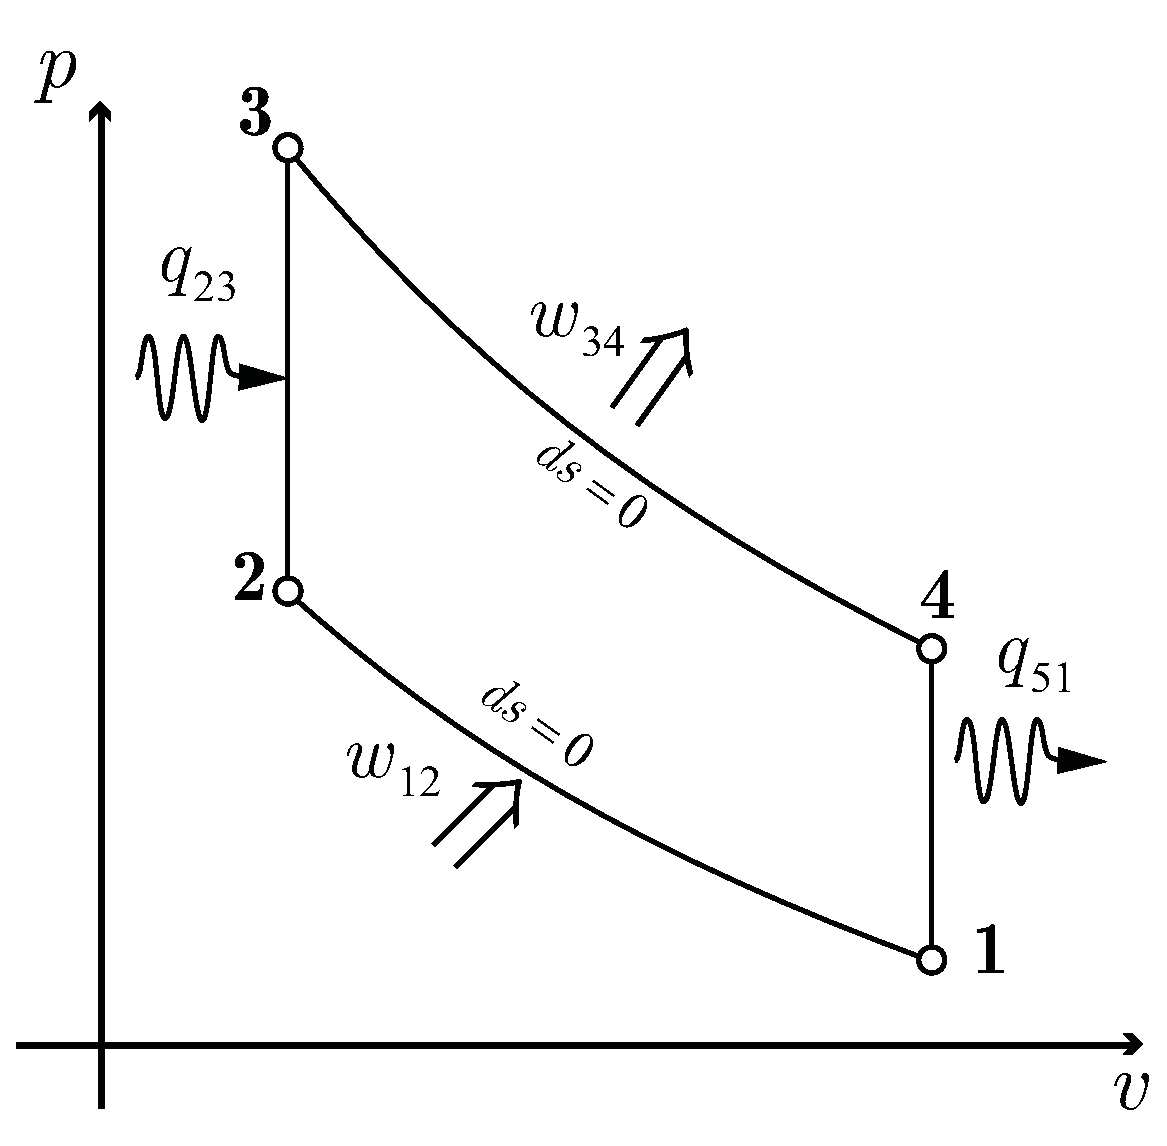
\includegraphics[width=8cm]{fig/ciclootto.eps}
    \caption{Ciclo Otto ideal. $q_{51}=q_{41}$}
    \label{fig:ottoideal}
\end{figure}

\subsection{Ciclo Diesel}

\begin{equation}
\eta_D=1-\frac{1}{\rc^{\ctegas-1}}\cdot\frac{\rv^k -1}{\ctegas(\rv-1)}
\end{equation}
donde $\rc=\frac{V_1}{V_2}$ y $\rv$ es la relación de \textit{cut-off} para el trayecto plano: $\rv=\frac{V_3}{V_2}>1$
\begin{figure}[htb!]
    \centering
    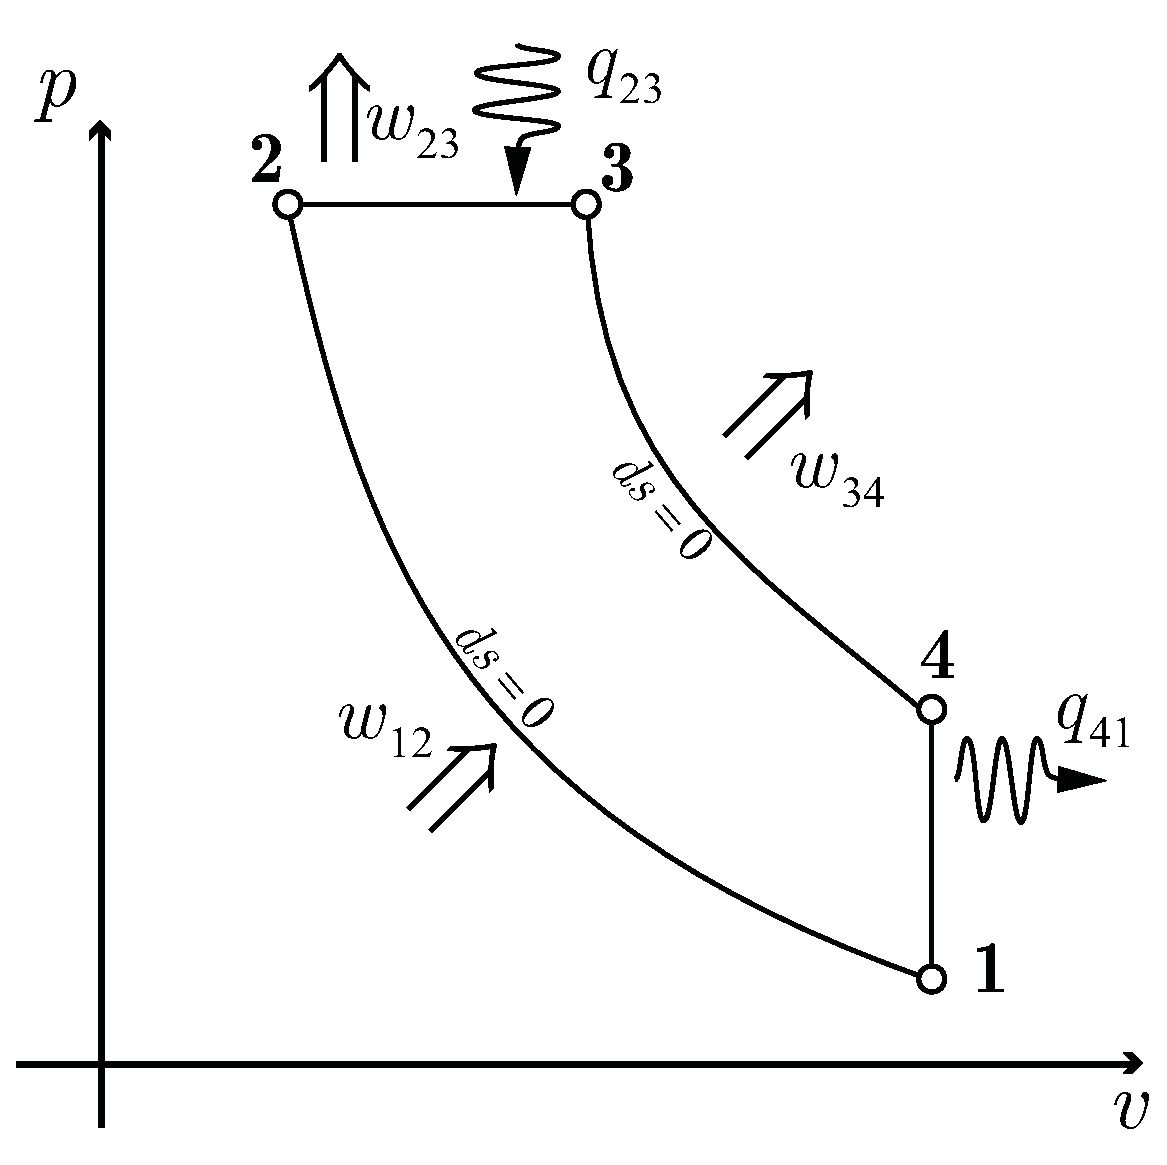
\includegraphics[width=10cm]{fig/ciclodiesel.eps}
    \caption{Ciclo Diesel ideal.}
    \label{fig:dieselideal}
\end{figure}

\subsection{Ciclo Dual o Sabathé}
También conocido com \textit{Diesel mixto}. 
\begin{equation}
\eta_S=1- \frac{T_5-T_1}{(T_3-T_2)+\ctegas(T_4-T_3)}
\end{equation}

\begin{equation}
\eta_S=1-\frac{1}{\rc^{\ctegas -1}}\cdot \frac{\rp(\rv)^\ctegas-1}{(\rp -1)+\ctegas\rp(\rv-1)}
\end{equation}
$\rc=\frac{V_1}{V_2}$, $\rv=\frac{V_4}{V_2}=\frac{V_4}{V_3}$ y $\rp=\frac{p_3}{p_2}=\frac{p_4}{p_2}$ es la relación de presiones en la etapa a volumen constante.
\begin{figure}[htb!]
    \centering
    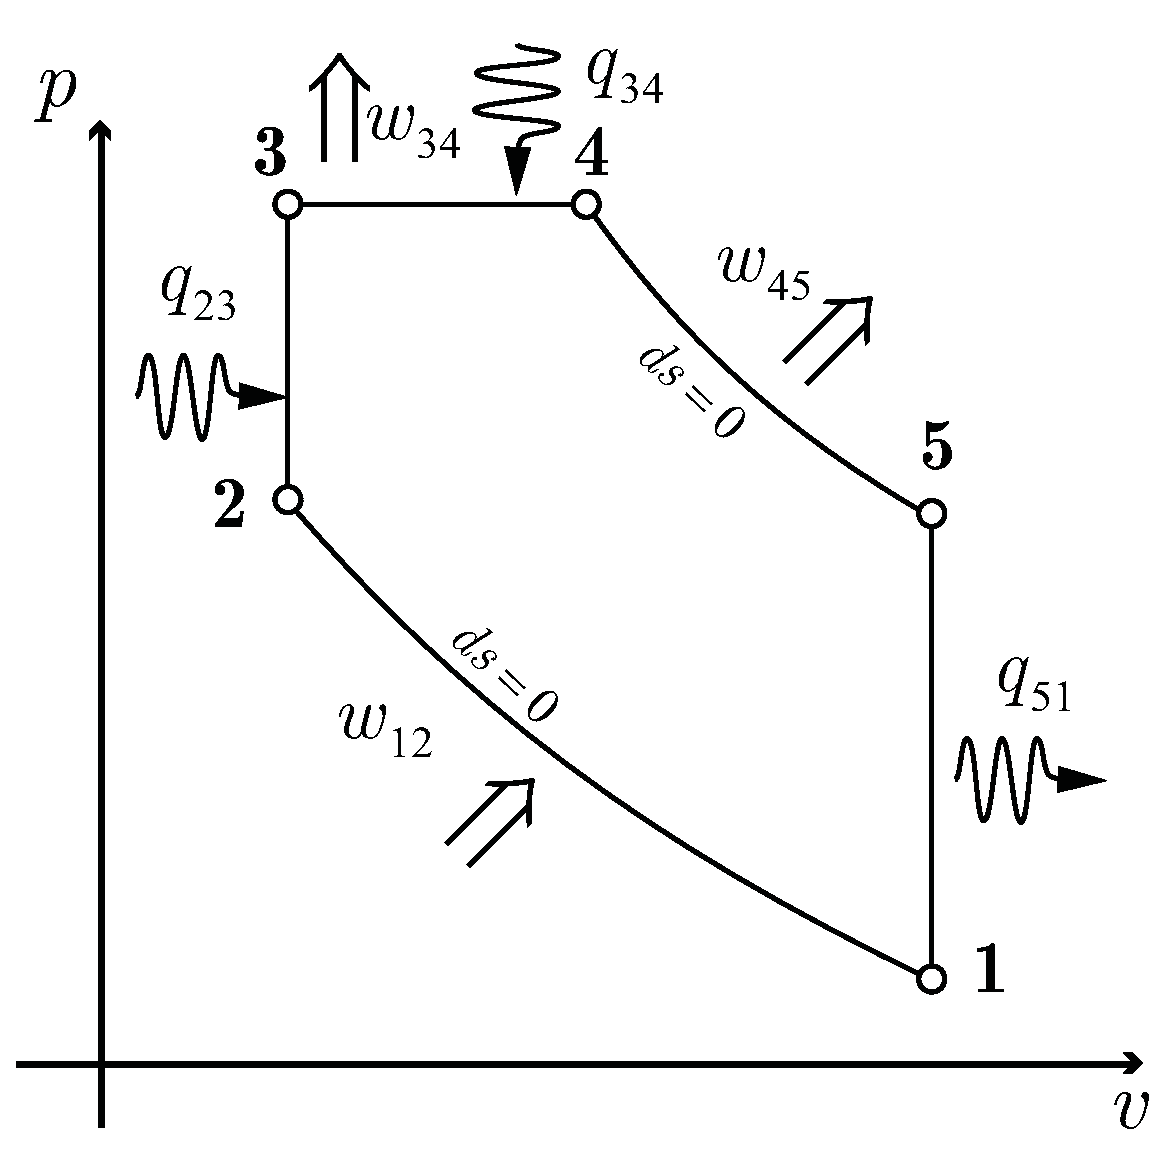
\includegraphics[width=10cm]{fig/ciclodual.eps}
    \caption{Ciclo Sabathé ideal.}
    \label{fig:dualideal}
\end{figure}


\end{document}
